\section{Architecture}

Diogenes has three main components:
an honesty checker for \coco,
an honesty checker for Java,
and an Eclipse plugin which integrates the two analyses
with an editor of \coco.
We illustrate the architecture of our tools in~\Cref{fig:architecture}.

\begin{figure}[t]
    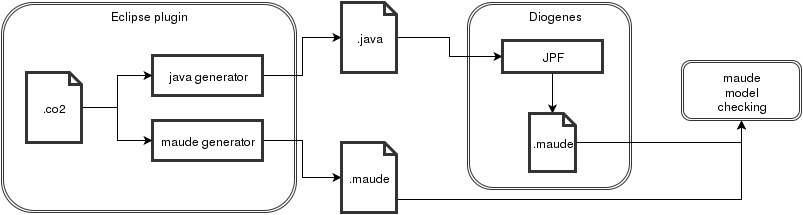
\includegraphics[width=\textwidth]{img/diogenes-arch.png}
    \caption{Data flow schema}
    \label{fig:architecture}
\end{figure}

The \coco honesty checker implements the  
verification technique introduced in~\cite{BMSZ15jlamp}.
This technique is built upon an abstract semantics of \coco 
which approximates both values (sent, received, and in conditional expressions) 
and the actual \emph{context} wherein a process is executed.
This abstraction is a \emph{sound} over-approximation of honesty:
namely, if the abstraction of a process is honest,
then also the concrete one is honest.
Further, in the fragment of \coco without conditional statements
the analysis is also \emph{complete},
\ie if a concrete process is honest, then also its abstraction is honest.
For processes without delimitation/parallel under process definitions,
the associate abstraction is finite-state, 
hence we can verify their honesty by model checking a (finite) state space.
For processes outside this class the analysis is still correct, 
but it may not terminate; indeed, a negative result in~\cite{BZ15wsfm}
excludes the existence of algorithm for honesty that are the same time
sound, complete, and terminating in full \coco.
% in all possible model of contracts which are at least as expressive
% as first-order binary session types~\cite{Honda98esop}.
Our implementation 
first translates a \coco process into a Maude term~\cite{Maude01}, 
and then uses the Maude LTL model checker~\cite{Eker02maude}
to decide honesty of its abstract semantics.


%\paragraph{Diogenes.}
The Java honesty checker is developed on top of \emph{Java PathFinder}
(JPF, \cite{lerda2001addressing,visser2003model}).
The JPF core is a Virtual Machine for Java bytecode
that can be configured to act as a model-checker.
%
A \emph{listener} allows us both to catch specific method invocations, 
which represent I/O actions
directed to the middleware~\cite{CO2middleware},
and to simulate \emph{all} the possible responses that 
the application can receive from it.
%
%JPF creates a \emph{choic explores all possible choices,
%and backtracks when a state exploration is done.
%
Therefore, the program is executed and backtracked multiple times,
and we are able to obtain a \coco model that represents its behaviour.
Then, the verification relies to the model checking technique of~\cite{BMSZ15jlamp}.
%
The accuracy of the model partially relies on the programmer:
the methods involved in the application logic have to be correctly annotated
and have to declare all possible exceptions that can be thrown at runtime.

The Eclipse plugin provides advanced functionalities such as
syntax highlighting, 
code auto-completion, 
outline view,
syntax/semantics checks,
and static type checking.
%
The plugin relies on
Xtext~\cite{xtext-site}, a framework for developing programming languages, 
and Xsemantics~\cite{xsemantics-site}, a domain-specific language for writing type systems
for Xtext-based languages.
%
We use Xtext to define the grammar of \coco
and we extend it to obtain custom semantic checks and adequate scope resolution of variables.

% We implement an Xtext grammar focusing on~\cite{BMSZ15jlamp},
% and we extend it in order to allow a complete mapping between \coco and Java.
